\documentclass[titlepage, 12pt]{article}

\usepackage{framed}
\usepackage{enumitem}
\usepackage{geometry}
\geometry{
  letterpaper,
  margin=1in,
}

\usepackage{graphicx}
\graphicspath{{./images/}}
\usepackage{float}

\title{SE 2XB3 Group 4 Report 3}
\author{
  Huang, Kehao \\
  400235182 \\
  \texttt{huangk53@mcmaster.ca} \\
  L01
  \and
  Jiao, Anhao \\
  400251837 \\
  \texttt{jiaoa3@mcmaster.ca} \\
  L01
  \and
  Ye, Xunzhou \\
  400268576 \\
  \texttt{yex33@mcmaster.ca} \\
  L01
}
\date{5 February 2021}

\begin{document}
\maketitle{}

\newpage{}

\section{Quicksort}

\subsection{In-Place Version}

Our implementation has its natural in-place advantage over the given
implementation which uses auxiliary memory to store different partitions for
each recursion call. Specifically, our in-place implementation swaps elements in
the array and uses two parameter \texttt{low} and \texttt{high} to mark the
array partition on which a recursion call should work. The amount of memory used
for the whole sorting process is independent of the input size. In this case, it
is the length of the input array. On the other hand, the given non-in-place
implementation copies elements from the input array to fresh allocated auxiliary
arrays. Each auxiliary array is used as the new partition for the subsequent
recursion call. And the returned sorted array is a concatenation of two sorted
partitions and the pivot. Both the element copying action and list concatenation
are costly, in terms of both time and space complexity.

A test on the average runtime of both versions of quicksort is then carried out.
For \( n \) on the scale from \( 10^4 \) to \( 10^7 \), an array of \( n \)
random numbers is passed to both implementations. The runtime is plotted on a
semi-log graph as shown in Figure \ref{fig:ip-ax}. The experimental result did
not precisely match our prediction. From \( n = 10^4 \) to approximately \( n =
10^{5.5} \), the in-place version has a slight longer runtime than the
non-in-place version. Figure \ref{fig:ip-ax-zoomed} is a zoomed-in view of the
plot, which demonstrates the shorter runtime of the non-in-place version. As \(
n \) increases from \( 10^{5.5} \), the in-place quicksort gradually starts to
outperform the other. The disadvantage of using auxiliary arrays and deep
copying data around memory becomes obvious as \( n \) passes \( 10^6 \).

\begin{figure}[h]
  \centering
  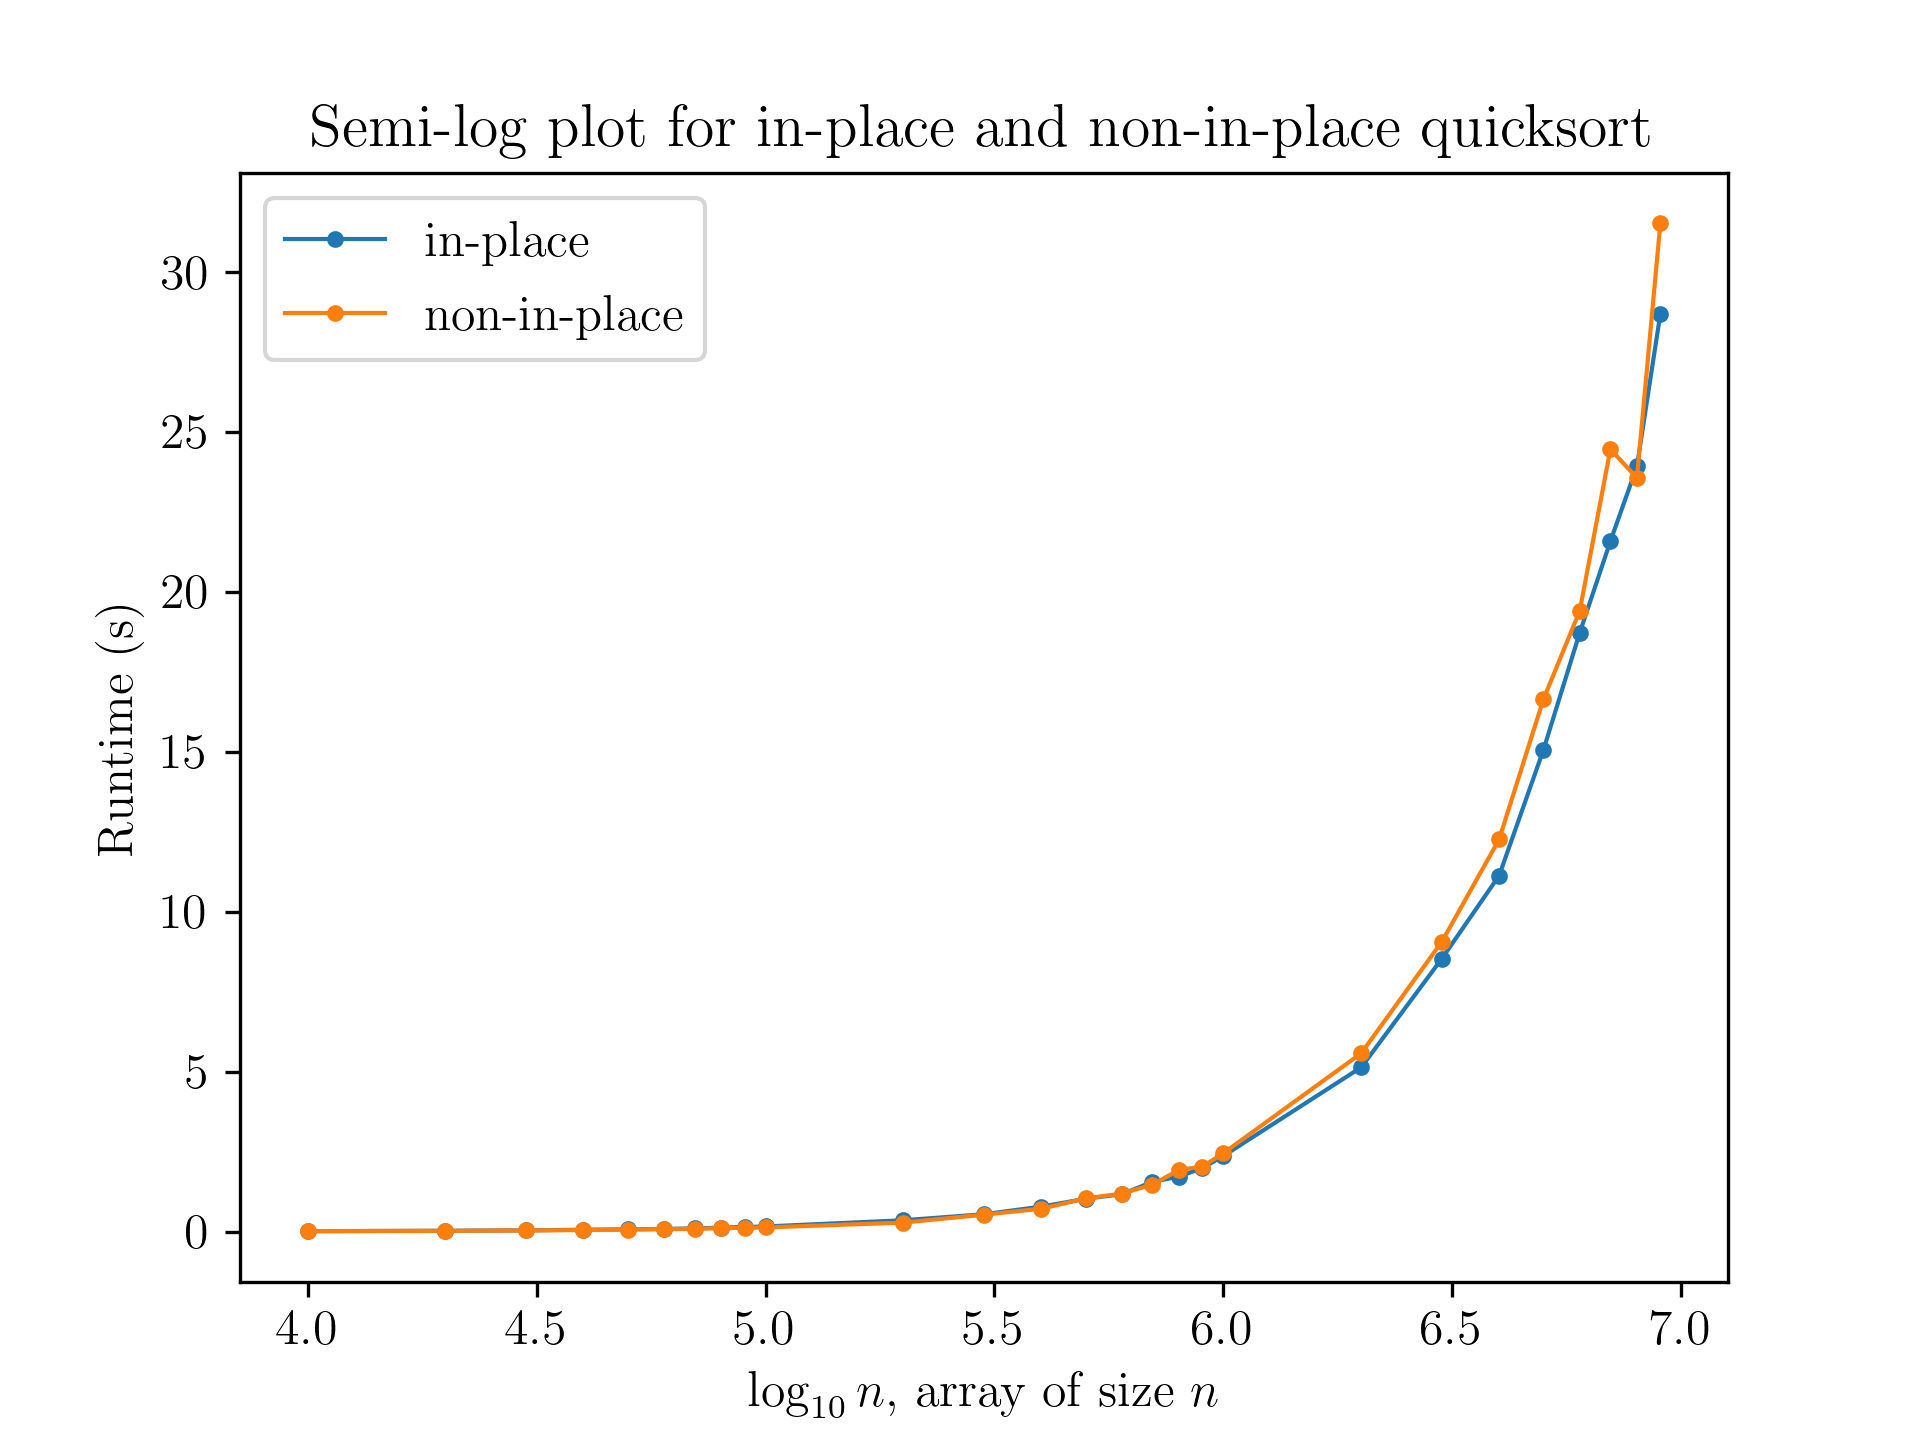
\includegraphics[width=0.8\textwidth]{ip-ax}
  \caption{In-place and non-in-place quicksort comparison}
  \label{fig:ip-ax}
\end{figure}
\begin{figure}[h]
  \centering
  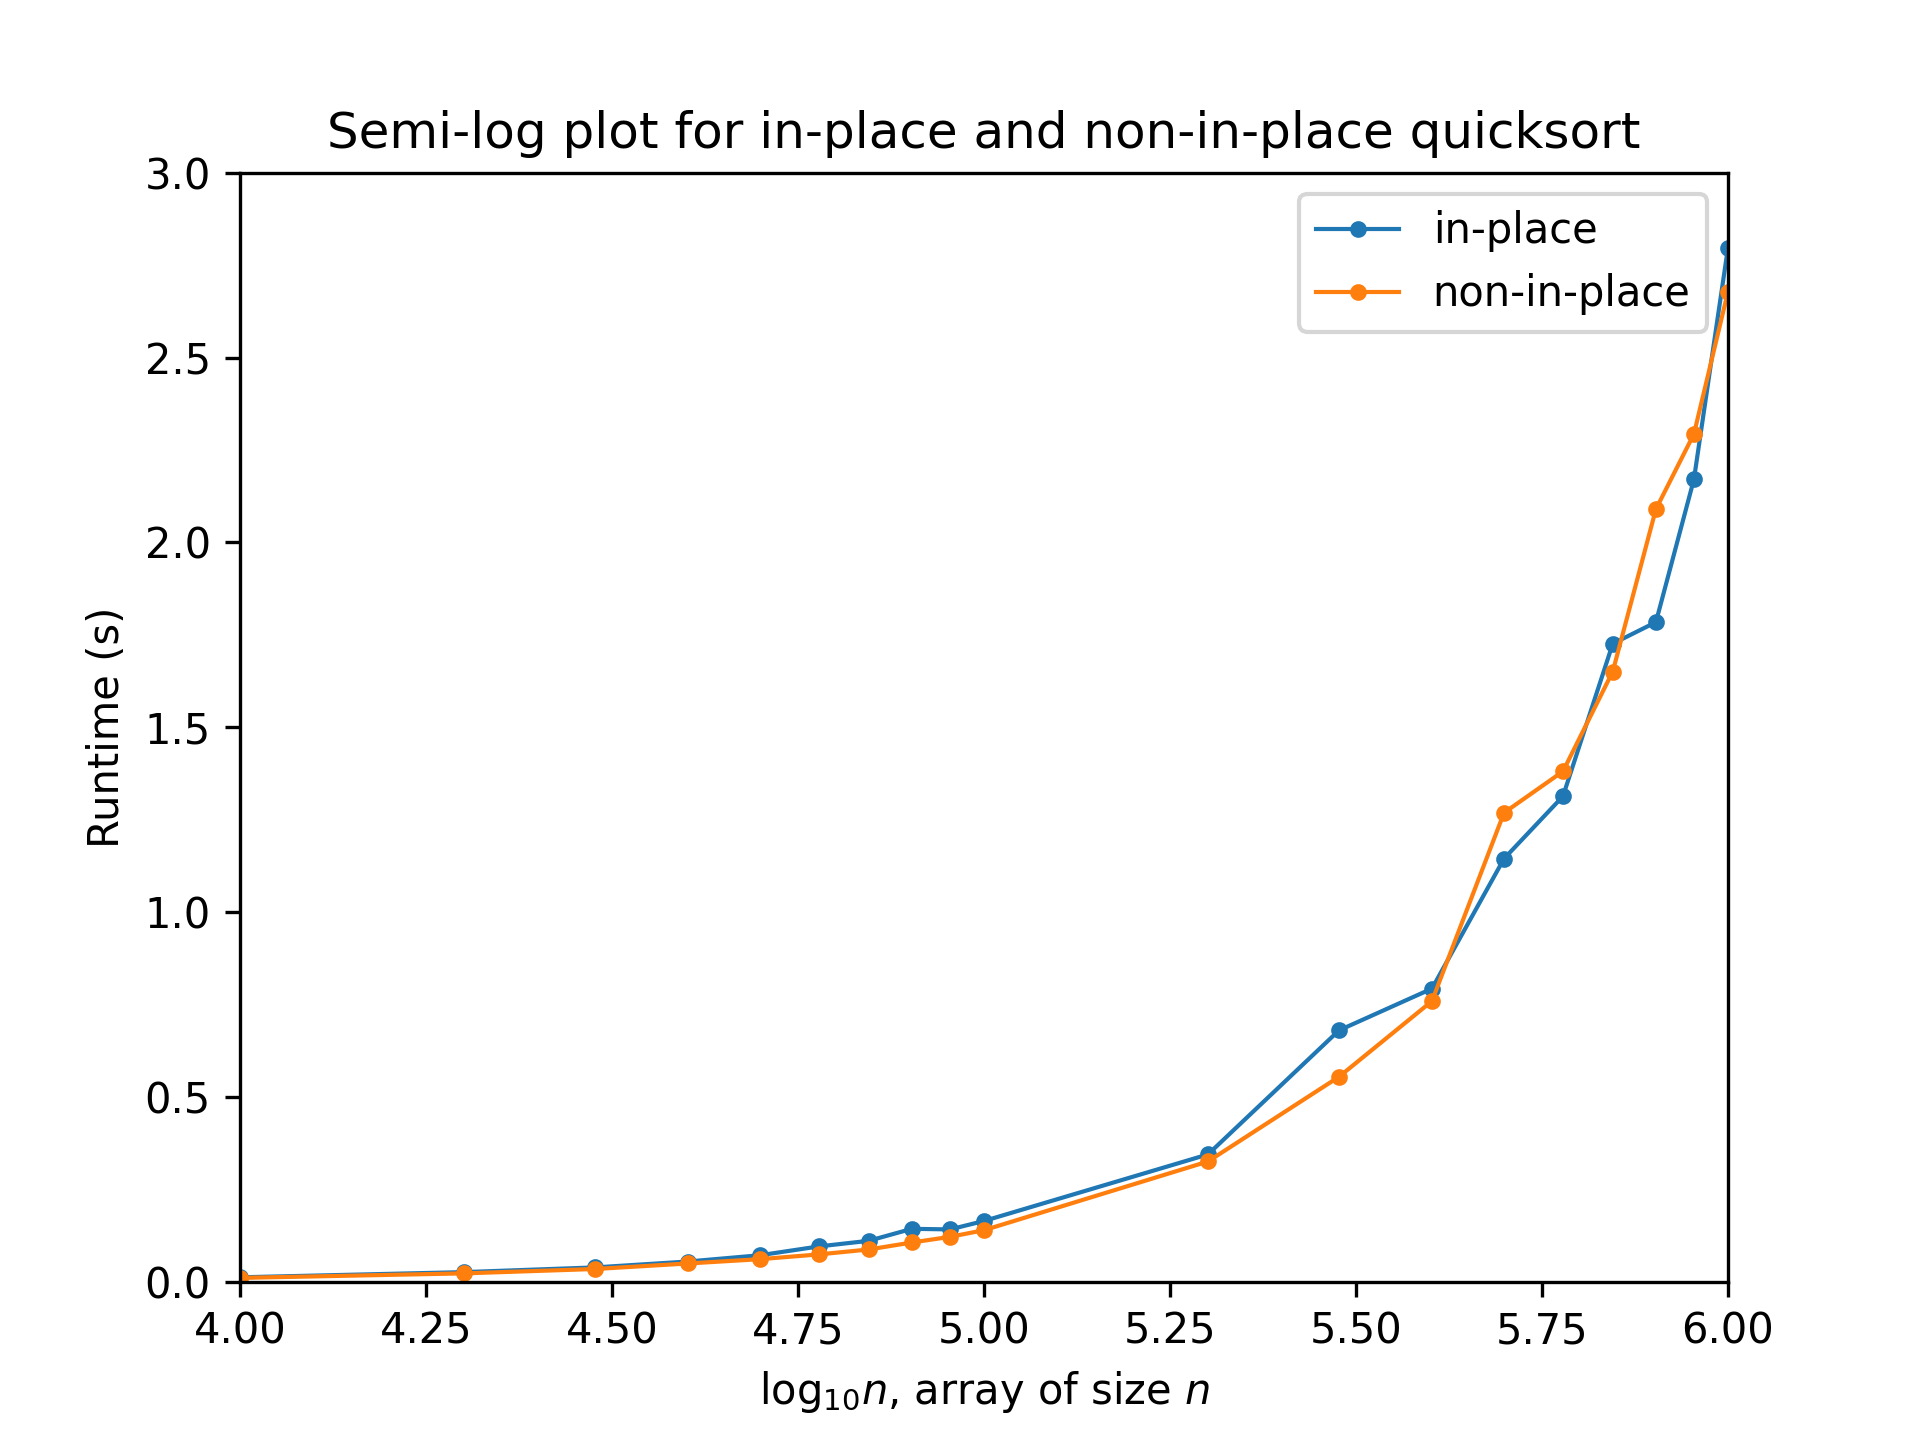
\includegraphics[width=0.8\textwidth]{ip-ax-zoomed} 
  \caption{Quicksort versions comparison on lower scale \( n \)}
  \label{fig:ip-ax-zoomed}
\end{figure}

To quantify the performance difference between the two versions, we used a
rather simple model. Either version of quicksort is known to have a complexity
of \( \mathcal{O}(n\lg{n}) \). We use \( c * n\lg{n} \) as an approximate model
of the imperial runtime. Thus we take the average of the differences of the \( c
\) constants of the two versions as the quantified performance difference. From
the same data set plotted above, for \( 10^4 \leq x < 10^6 \), the non-in-place
version is on average 4\% faster than the in-place version.

In conclusion, the non-in-place quicksort is slightly faster than the in-place
one in practice. However, the in-place version has an observable speed
improvement for an input size \( n > 10^6 \).

\end{document}
